\section{Simple List Data Sets}\label{simple-list-data-sets}

\subsection{AirCooledChillers.idf}\label{aircooledchillers.idf}

This dataset includes performance curves for air cooled electric EIR chiller (object type: Chiller:Electric:EIR). Knowing the type of chiller that you want to simulate, you can find it and the associated performance curves in the dataset file. A brief synopsis of AirCooledChiller.idf is shown below:

\begin{lstlisting}

! AirCooledChillers.idf
  !
  ! This dataset includes performance curves for object type Chiller:Electric:EIR
  !
  ! Summary Table for Electric EIR Chiller reference data sets.
  ! Chillers are listed in order of reference capacity. Reference capacity and COP do not necessarily
  ! indicate rated capacity and COP at standard rating conditions (e.g. ARI Standard 550/590).
  !
  ! Performance curves developed from information collected from manufacturer's catalog data
  ! The nomenclature used for the chiller is as follows:
  ! ElectricEIRChiller - Manufacturer's Name - Model - Reference Capacity in kW - Reference COP
  !
  !                                                      Compressor   Reference    Reference
  ! Chiller Name                                            Type       Capacity      COP
  !                                                                    kW (tons)
  ! ElectricEIRChiller McQuay AGZ010BS 34.5kW/2.67COP      Scroll     34.5 (9.8)      2.67
  ! ElectricEIRChiller McQuay AGZ013BS 47.1kW/2.67COP      Scroll     47.1 (13.4)     2.67
  ! ElectricEIRChiller York YCAL0019EE 54.2kW/2.9COP       Scroll     54.2 (15.4)     2.9
  ! ElectricEIRChiller McQuay AGZ017BS 54.5kW/2.67COP      Scroll     54.5 (15.5)     2.67
\end{lstlisting}

\subsection{ASHRAE\_2005\_HOF\_Materials.idf}\label{ashraeux5f2005ux5fhofux5fmaterials.idf}

This reference data set contains content from two chapters in the ASHRAE 2005 Handbook of Fundamentals, Chapter 30 - the Cooling and Heating Loads calculations chapter has both materials with thermal properties and constructions for Light, Medium, and Heavy buildings. Chapter 25 contains details thermal properties of many materials -- no constructions are created from that data.

The following materials and constructions are created from ASHRAE Handbook of Fundamentals, 2005, Chapter 30, Table 19 and Table 22. These are representative of materials and constructions used in Cooling and Heating Load Calculations.

\subsection{Boilers.idf}\label{boilers.idf}

This dataset includes performance curves for non-electric boilers. Reference: Condensing Technology, Technical Series, Viessmann, 9446 803 - 1 GB Nov. 2004.

\subsection{California\_Title\_24-2008.idf}\label{californiaux5ftitleux5f24-2008.idf}

This dataset includes occupancy data and non-residential schedules for California Title 24-2008 compliance calculations when lighting plans are submitted for the Entire Building or when lighting compliance is not performed. Data is based on Table N2-5 of the 2008 Non-residential ACM Manual.

\subsection{Chillers.idf}\label{chillers.idf}

This dataset includes object types for specific (by manufacturer and type) Chiller:Electric:EIR and Chiller: Electric:ReformulatedEIR and associated performance curves.

Knowing the type of chiller that you want to simulate, you can find it and the associated performance curves in the dataset file. By example, here is part of the comments in the Chiller.idf file:

\begin{lstlisting}

! Summary Table for Electric EIR Chiller reference data sets (Ref. CoolTools project).
  ! Chillers are listed in order of compressor type and reference capacity (model calibration
  ! point). Reference capacity and COP do not necessarily indicate rated capacity and COP at
  ! standard rating conditions (e.g. ARI Standard 550/590).
  !
  ! Performance curves developed from information collected over a 10-year period from 1991 to 2001.
  !
  !                                                      Compressor   Reference  Reference Unloading
  ! Chiller Name                                            Type       Capacity    COP     Mechanism
  !                                                                    kW (tons)
  !-------------------------------------------------------------------------------------------------
  ! ElectricEIRChiller McQuay WSC 471kW/5.89COP/Vanes    Centrifugal   471 (134)   5.89   Inlet Vanes
  ! ElectricEIRChiller York YT 563kW/10.61COP/Vanes      Centrifugal   563 (160)   10.61  Inlet Vanes
  ! ElectricEIRChiller McQuay PEH 703kW/7.03COP/Vanes    Centrifugal   703 (200)   7.03   Inlet Vanes
  ! ElectricEIRChiller Carrier 23XL 724kW/6.04COP/Vanes  Centrifugal   724 (206)   6.04   Inlet Vanes
\end{lstlisting}

\subsection{CodeCompliantEquipment.idf}\label{codecompliantequipment.idf}

This dataset includes performance curve objects that describe the part load performance of building energy code minimally compliant equipment. The dataset provides curves for the following EnergyPlus objects: Chiller:Electric:EIR. Sets of curves are provided for the following building energy codes minimum requirements: ASHRAE Standard 90.1-2019 Table 6.8.1-3, ASHRAE Standard 90.1-2019 Table G3.5.3.

Generating performances curves meeting both full and part load efficiency numbers require solving a largely underdetermined system of equations. The number of unknowns depend on the type of curves, which mostly depend on the algorithm used by the software and used in models. It also means that an infinite number of solutions exists. One way to solve this issue is to turn it into a constrained problem and use a simple genetic algorithm (GA) with a well-defined objective or cost function to determine potential solutions with physical significance. A GA can have a short computational time, be scalable, versatile, find solutions to problems with large number of parameters to problems with multiple local optima so it is a good candidate for this task. The algorithm used to generate the curves in this dataset starts with a ``seed'' set of curves that can be user-modifiable, target full load, and part load efficiency as inputs.

Among others, a ``nearest neighbor'' type method was developed to aggregate sets of curves and generate a generic set of curves for a specific target to be used as ``seed'' set of curves to the aforementioned algorithm. This method selects the N sets of performance curves that best match the targeted equipment characteristics in terms of capacity, full load efficiency, part load efficiency, and other applicable characteristics. Each selected sets of curves are scored based on how close it is to the targeted equipment characteristics. A wide mesh of values for each input variable(s) to each curve is then created and corresponding output calculated. The outputs are then weighted average based on their previously determined score. A regression and normalization at rated conditions is then performed to obtain the aggregated curves.

\begin{lstlisting}

!----------------------------------------------------------
!- Beginning of performance curves for Chiller:Electric:EIR:

Curve:Quadratic,
    ASHRAE901_AppG_wtr_cent_gte150lt300ton_0.634kWpton_0.596IPLV.IP_eir-f-plr,    !- Name
    0.30662667381140624,      !- Coefficient1 Constant
    0.06295923908320235,      !- Coefficient2 x
    0.6358315679053916,       !- Coefficient3 x2
    0.0,                      !- Minimum Value of x
    1.0,                      !- Maximum Value of x
    ,                         !- Minimum Curve Output
    ;                         !- Maximum Curve Output
  
\end{lstlisting}

\subsection{CompositeWallConstructions.idf}\label{compositewallconstructions.idf}

The Reference Data Set CompositeWallConstructions.idf contains constructions and associated materials for a set of \textbf{composite} walls. These are walls---such as stud walls---that have complicated heat-flow paths so that the conduction is two- or three-dimensional.

An example entry in this data set--for an insulated 2''x4'' steel-stud wall--looks like:

\begin{lstlisting}

CONSTRUCTION,Composite 2x4 Steel Stud R11,
  ! ASHRAE 1145-RP Wall Assembly 10
  ! 2"x4" steel studs at 24" on center with between-stud R11 fibreglass insulation.
  ! Studs are 3.5", 16 gauge, 15 flange.
  ! Layers are 1/2" wood siding, 1/2" plywood, 2x4 steel studs and R11 insulation, 1/2" gypsum board.
  ! Area-average R-Value = 8.796 ft2-F-h/Btu (1.548 m2-K/W).
  ! Total wall thickness = 5.00in (0.127m)
  ! Material layer names follow:
    Composite 2x4 Steel Stud R11 \#3,
    Composite 2x4 Steel Stud R11 \#2,
    Composite 2x4 Steel Stud R11 \#1;
  MATERIAL,Composite 2x4 Steel Stud R11 \#1,
    Smooth,  !- Roughness
    0.013,   !- Thickness (m)
    0.720,   !- Conductivity (W/m-K)
    640.0,   !- Density (kg/m3)
    1048,    !- Specific Heat (J/kg-K)
    0.9,     !- Absorptance:Thermal
    0.7,     !- Absorptance:Solar
    0.7;     !- Absorptance:Visible
  MATERIAL,Composite 2x4 Steel Stud R11 \#2,
    Smooth,  !- Roughness
    0.089,   !- Thickness (m)
    0.060,   !- Conductivity (W/m-K)
    118.223, !- Density (kg/m3)
    1048,    !- Specific Heat (J/kg-K)
    0.9,     !- Absorptance:Thermal
    0.7,     !- Absorptance:Solar
    0.7;     !- Absorptance:Visible
  MATERIAL,Composite 2x4 Steel Stud R11 \#3,
    Smooth,  !- Roughness
    0.025,   !- Thickness (m)
    0.452,   !- Conductivity (W/m-K)
    413.782, !- Density (kg/m3)
    1048,    !- Specific Heat (J/kg-K)
    0.9,     !- Absorptance:Thermal
    0.7,     !- Absorptance:Solar
    0.7;     !- Absorptance:Visible
\end{lstlisting}

The materials here are \textbf{not} real materials but are ``equivalent'' materials obtained from finite-difference modeling. The thickness, conductivity, density and specific heat values of the material layers for the different constructions have been taken from the ASHRAE report ``Modeling Two- and Three-Dimensional Heat Transfer through Composite Wall and Roof Assemblies in Hourly Energy Simulation Programs (1145-TRP),'' by Enermodal Engineering Limited, Oak Ridge National Laboratory, and the Polish Academy of Sciences, January 2001. EnergyPlus will calculate conduction transfer functions using these materials. The heat transfer based on these conduction transfer functions will then be very close to what would be calculated with a two- or three-dimensional heat transfer calculation.

For stud walls, using these composite constructions will give more accurate heat flow than you would get by manually dividing the wall into a stud section and a non-stud section.

If your wall's exterior or interior roughness or thermal, solar or visible absorptances are different from those in the data set, you can make the appropriate changes to the first material (the outside layer) or the third material (the inside layer). \textbf{None of the other values should be changed.}

Following is a summary of the constructions in the composite wall data set:

\begin{lstlisting}

CONSTRUCTION,Composite 2x4 Wood Stud R11,
  ! ASHRAE 1145-RP Wall Assembly 1
  ! 2"x4" wood studs at 24" on center with between-stud R11 fibreglass insulation.
  ! Layers are 1/2" wood siding, 1/2" plywood, 2x4 wood studs and R11 insulation, 1/2" gypsum board.
  ! Area-average R-Value = 11.391 ft2-F-h/Btu (2.005 m2-K/W).

  CONSTRUCTION,Composite 2x6 Wood Stud R19,
  ! ASHRAE 1145-RP Wall Assembly 2
  ! 2"x6" wood studs at 24" on center with between-stud R19 fibreglass insulation.
  ! Layers are 1/2" wood siding, 1/2" plywood, 2x6 wood studs and R19 insulation, 1/2" gypsum board.
  ! Area-average R-Value = 17.487 ft2-F-h/Btu (3.078 m2-K/W).

  CONSTRUCTION,Composite Insulated Concrete Form Wall With Steel Ties,
  ! ASHRAE 1145-RP Wall Assembly 7
  ! Wall system is made of two rigid insulation sides held together with wire mesh.
  ! The two sides come together to create the formwork for the concrete.
  ! Layers are 3/4" concrete stucco, outer polystyrene shell, concrete core, inner polystyrene shell.
  ! Area-average R-Value = 11.230 ft2-F-h/Btu (1.977 m2-K/W).

  CONSTRUCTION,Composite Concrete/Foam/Concrete With Steel Connectors,
  ! ASHRAE 1145-RP Wall Assembly 8
  ! Wall system is made of two 3" concrete slabs separated by 2" rigid insulation.
  ! The slab connectors are steel ties with a 0.15"x0.15" cross section.
  ! Layers are 3" concrete, 2" polystyrene, 3" concrete.
  ! Area-average R-Value = 7.659 ft2-F-h/Btu (1.348 m2-K/W).

  CONSTRUCTION,Composite Concrete/Foam/Concrete With Plastic Connectors,
  ! ASHRAE 1145-RP Wall Assembly 9
  ! Wall system is made of two 3" concrete slabs separated by 2" rigid insulation.
  ! The slab connectors are plasic ties with a 0.25"x0.25" cross section.
  ! Layers are 3" concrete, 2" polystyrene, 3" concrete.
  ! Area-average R-Value = 10.582 ft2-F-h/Btu (1.862 m2-K/W).

  CONSTRUCTION,Composite 2x4 Steel Stud R11,
  ! ASHRAE 1145-RP Wall Assembly 10
  ! 2"x4" steel studs at 24" on center with between-stud R11 fibreglass insulation.
  ! Studs are 3.5", 16 gauge, 15 flange.
  ! Layers are 1/2" wood siding, 1/2" plywood, 2x4 steel studs and R11 insulation, 1/2" gypsum board.
  ! Area-average R-Value = 8.796 ft2-F-h/Btu (1.548 m2-K/W).

  CONSTRUCTION,Composite Brick Foam 2x4 Steel Stud R11,
  ! ASHRAE 1145-RP Wall Assembly 15
  ! Brick veneer, polystyrene, 2"x4" steel studs at 24" on center with
  !  between-stud R11 fibreglass insulation.
  ! Studs are 3.5", 16 gauge, 15 flange.
  ! Layers are 3.25" brick,1" polystyrene insulation, 1/2" plywood, 2x4 steel studs and R11 insulation,
  !  1/2" gypsum board.
  ! Area-average R-Value = 12.792 ft2-F-h/Btu (2.251 m2-K/W).

  CONSTRUCTION,Composite 2x6 Steel Stud R19,
  ! ASHRAE 1145-RP Wall Assembly 16
  ! 2"x6" steel studs at 24" on center with between-stud R19 fibreglass insulation.
  ! Studs are 5.5", 16 gauge, 15 flange.
  ! Layers are 1/2" wood siding, 1/2" plywood, 2x6 steel studs and R19 insulation, 1/2" gypsum board.
  ! Area-average R-Value = 12.792 ft2-F-h/Btu (1.991 m2-K/W).

  CONSTRUCTION,Composite Foam 2x6 Steel Stud R19,
  ! ASHRAE 1145-RP Wall Assembly 17
  ! Polystyrene, 2"x6" steel studs at 24" on center with between-stud R19 fibreglass insulation.
  ! Studs are 5.5", 16 gauge, 15 flange.
  ! Layers are 3/4" concrete stucco,1" polystyrene insulation, 1/2" plywood, 2x6 steel studs and R19 insulation,
  !  1/2" gypsum board.
  ! Area-average R-Value = 15.157 ft2-F-h/Btu (2.668 m2-K/W).

  CONSTRUCTION,Composite Brick Foam 2x6 Steel Stud R19,
  ! ASHRAE 1145-RP Wall Assembly 18
  ! Brick veneer, polystyrene, 2"x6" steel studs at 24" on center with
  !  between-stud R19 fibreglass insulation.
  ! Studs are 5.5", 16 gauge, 15 flange.
  ! Layers are 3.25" brick,1" polystyrene insulation, 1/2" plywood, 2x6 steel studs and R19 insulation,
  !  1/2" gypsum board.
  ! Area-average R-Value = 15.465 ft2-F-h/Btu (2.722 m2-K/W).

  CONSTRUCTION,Composite 2-Core Filled Concrete Block Uninsulated,
  ! ASHRAE 1145-RP Wall Assembly 19
  ! Wall system is made of 12" 2-core concrete blocks without insulation.
  ! The core area is filled with rebar and poured concrete.
  ! Area-average R-Value = 1.326 ft2-F-h/Btu (0.239 m2-K/W).

  CONSTRUCTION,Composite 2-Core Filled Concrete Block Insulated,
  ! ASHRAE 1145-RP Wall Assembly 20
  ! Wall system is made of 12" 2-core concrete blocks with 1.875"-thick
  !  foam inserts in the block cores.
  ! The remaining core area is filled with poured concrete.
  ! Area-average R-Value = 2.291 ft2-F-h/Btu (0.403 m2-K/W).
\end{lstlisting}

\subsection{DXCoolingCoil.idf}\label{dxcoolingcoil.idf}

This dataset includes performance curves for the object types Coil:Cooling:DX:SingleSpeed and Coil:Cooling:DX:TwoStageWithHumidityControlMode. This data set is developed by using catalog data published by different manufacturers which are listed in the file.

Here is a synopsis of the DXCoolingCoil.idf:

\begin{lstlisting}

! DXCoolingCoil.idf
  !
  ! This dataset includes performance curves for the object types Coil:Cooling:DX:SingleSpeed and
  ! Coil:Cooling:DX:TwoStageWithHumidityControlMode
  !
  ! Reference capacity at standard rating conditions (ARI 95F OAT, 67F EWBT and air flow rate
  ! around 400 cfm/Ton).
  !
  ! In the objects Coil:Cooling:DX:SingleSpeed and Coil:Cooling:DX:TwoStageWithHumidityControlMode
  ! below, input fields 'Availability Schedule Name', 'Air Inlet Node Name' and 'Air Outlet Node
  ! Name' need to be defined by the user.
  !
  !------------------------------------------------------------------------------------------------!                             Compressor  Nominal    Reference      Reference   Refrig  Expansion
  !                                                                                         Valve
  ! Name                           Type     Capacity   Capacity          COP       Type      Type
  !                                         (tons)     kW (tons)
  !------------------------------------------------------------------------------------------------! Carrier Centurion 50PG06      Scroll      5        18.28(5.2)        4.15     R-410A    TXV
  ! Carrier Centurion 50PG12      Scroll      10       36.79(10.47)      4.05     R-410A    TXV
  ! Carrier Centurion 50PG24      Scroll      20       73.81(21)         3.95     R-410A    TXV

    Coil:Cooling:DX:SingleSpeed,
      Carrier Centurion 50PG06,     !- Name
      CoolingCoilAvailSched,        !- Availability Schedule Name
      18276.96,                     !- Rated Total Cooling Capacity {W}
      0.74,                         !- Rated Sensible Heat Ratio
      4.15,                         !- Rated COP
      0.944,                        !- Rated Air Flow Rate {m3/s}
      ,                             !- Rated Evaporator Fan Power Per Volume Flow Rate {W/(m3/s)}
      DXCoilAirInletNode,           !- Air Inlet Node Name
      DXCoilAirOutletNode,          !- Air Outlet Node Name
      CarrierCenturion50PG06CapFT,  !- Total Cooling Capacity Function of Temperature Curve Name
      CarrierCenturion50PG06CapFFF, !- Total Cooling Capacity Function of Flow Fraction Curve Name
      CarrierCenturion50PG06EIRFT,       !- Energy Input Ratio Function of Temperature Curve Name
      CarrierCenturion50PG06EIRFFF,      !- Energy Input Ratio Function of Flow Fraction Curve Name
      Carrier Centurion 50PG06 PLFFPLR;  !- Part Load Fraction Correlation Curve Name

  ! Curve set (5 Curves):

  ! Cooling Capacity Function of Temperature Curve
  ! x = Entering Wet-bulb Temp and y = Outdoor Dry-bulb Temp

    Curve:Biquadratic,
      CarrierCenturion50PG06CapFT,  !- Name
      0.9953455,               !- Coefficient1 Constant
      -0.0118418,              !- Coefficient2 x
      0.0012277,               !- Coefficient3 x**2
      0.0030246,               !- Coefficient4 y
      -0.0000702,              !- Coefficient5 y**2
      -0.0003685,              !- Coefficient6 x*y
      12.22,                   !- Minimum Value of x
      26.67,                   !- Maximum Value of x
      15.56,                   !- Minimum Value of y
      51.67,                   !- Maximum Value of y
      ,                        !- Minimum Curve Output
      ,                        !- Maximum Curve Output
      Temperature,             !- Input Unit Type for X
      Temperature,             !- Input Unit Type for Y
      Dimensionless;           !- Output Unit Type

  ! EIR Function of Temperature Curve
  ! x = Entering Wet-bulb Temp and y = Outdoor Dry-bulb Temp

    Curve:Biquadratic,
      CarrierCenturion50PG06EIRFT,  !- Name
      0.3802131,               !- Coefficient1 Constant
      0.0199468,               !- Coefficient2 x
      -0.0006682,              !- Coefficient3 x**2
      0.0058933,               !- Coefficient4 y
      0.0004646,               !- Coefficient5 y**2
      -0.0004072,              !- Coefficient6 x*y
      12.22,                   !- Minimum Value of x
      26.67,                   !- Maximum Value of x
      15.56,                   !- Minimum Value of y
      51.67,                   !- Maximum Value of y
      ,                        !- Minimum Curve Output
      ,                        !- Maximum Curve Output
      Temperature,             !- Input Unit Type for X
      Temperature,             !- Input Unit Type for Y
      Dimensionless;           !- Output Unit Type

  ! Cooling Capacity Function of Flow Fraction Curve
  ! x = Flow Fraction

    Curve:Quadratic,
      CarrierCenturion50PG06CapFFF,  !- Name
      0.7705358,               !- Coefficient1 Constant
      0.2848007,               !- Coefficient2 x
      -0.0580891,              !- Coefficient3 x**2
      0.75,                    !- Minimum Value of x
      1.25;                    !- Maximum Value of x

  ! EIR Function of Flow Fraction Curve
  ! x = Flow Fraction

    Curve:Quadratic,
      CarrierCenturion50PG06EIRFFF,   !- Name
      1.3439758,               !- Coefficient1 Constant
      -0.5111244,              !- Coefficient2 x
      0.1732549,               !- Coefficient3 x**2
      0.75,                    !- Minimum Value of x
      1.25;                    !- Maximum Value of x

  ! Part Load Fraction Function of Part Load Ratio Curve
  ! x = Part Load Ratio

    Curve:Quadratic,
      CarrierCenturion50PG06PLFFPLR,   !- Name
      0.85,                    !- Coefficient1 Constant
      0.15,                    !- Coefficient2 x
      0.0,                     !- Coefficient3 x**2
      0.0,                     !- Minimum Value of x
      1.0;                     !- Maximum Value of x
\end{lstlisting}

\subsection{ElectricGenerators.idf}\label{electricgenerators.idf}

This dataset includes inputs for the GENERATOR:MICROTURBINE object and associated performance curves. The performance curves were developed from manufacturer data collected in Summer 2007.

Includes data for generators: Capstone C65, Elliott TA100,~ Ingersoll Rand MT70, Ingersoll Rand MT250.

Further documentation is contained in the dataset file.

\subsection{Electricity USA Environmental Impact Factors.idf}\label{electricity-usa-environmental-impact-factors.idf}

United States 1999 national average electricity emissions factors based on eGRID, 1605, AirData. United States Water Emission Fuel Factors are the combined thermoelectric and hydroelectric weighted averages from:

Torcellini, Paul; Long, Nicholas; Judkoff, Ron; ``Consumptive Water Use for U.S. Power Production'';NREL Report No. TP-550-33905. Golden, CO; 2003; \url{http://www.nrel.gov/docs/fy04osti/33905.pdf};

or

Torcellini, Paul; Long, Nicholas; Judkoff, Ron; ``Consumptive Water Use for U.S. Power Production''; ASHRAE Transactions 2003, Vol 110, Part 1. Atlanta, GA; January 2004;

\subsection{ElectronicEnthalpyEconomizerCurves.idf}\label{electronicenthalpyeconomizercurves.idf}

These curves approximate the electronic (variable) enthalpy curves used to simulate humidity biased economizer control. This control scheme adjusts the upper outdoor air humidity ratio based on outdoor air dry-bulb temperature as shown in the figure below. California Title 24 ACM 2005 lists the optional economizer control strategies. One of these control strategies is referred to as variable enthalpy control curve A. This control strategy is also cited in ASHRAE Standard 90.1-2004, using the term ``electronic enthalpy''. Electronic enthalpy curves A-D are included in this dataset.

\begin{figure}[hbtp] % fig 12
\centering
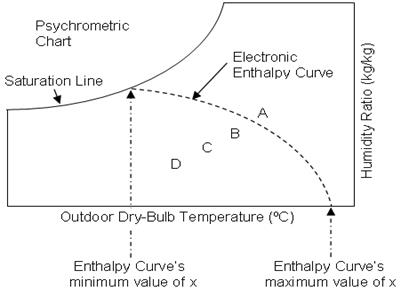
\includegraphics[width=0.9\textwidth, height=0.9\textheight, keepaspectratio=true]{media/image027.jpg}
\caption{Psychrometric Chart Illustration of the Electronic (Variable) Enthalpy Economizer Limit Example Curve Objects \protect \label{fig:psychrometric-chart-illustration-of}}
\end{figure}

For the curves provided, curve A has the highest limit and curve D has the lowest limit. These curve objects represent a single-point electronic enthalpy control curve with the curve object's minimum value of x (temperature) crossing the psychrometric chart's saturation line and the curve object's maximum value of x crossing the psychrometric chart's dry-bulb temperature axis. The curve object's minimum (maximum) value of x should be just low (high) enough to ensure that the curve crosses the psychrometric chart's saturation line (temperature axis). The curves are evaluated at an outdoor dry-bulb temperature to provide a maximum operating outdoor humidity ratio for economizer operation. If the outdoor humidity ratio is greater than this maximum value, economizer operation is terminated. These curves may be used with other economizer limits to create multi-point economizer control (Temperature Limit, Temperature Low Limit, Enthalpy Limit, and Dewpoint Temperature Limit).

\subsubsection{Form of the Electronic Enthalpy Curve Equation:}\label{form-of-the-electronic-enthalpy-curve-equation}

The electronic enthalpy curve equation represents a unique curve and is a function of both temperature and relative humidity. The equation is set equal to a constant which provides a unique temperature for each relative humidity entered into the equation. Each control curve has a unique constant as shown in the table below. Other constants may be used to develop specialized electronic enthalpy curves.

\begin{equation}
K = 45.672192 - 1.1559942 \cdot T - 0.144599 \cdot RH
\end{equation}

where:

\begin{itemize}
\tightlist
\item
  K~ = Constant value to represent specific curve
\item
  T~ = Outdoor Dry-Bulb Temperature (C)
\item
  RH = Outdoor Relative Humidity (\%)
\end{itemize}

NOTE:~ modifying the RH multiplier (-0.144599) tends to ``wag'' the curvature at the upper relative humidities. Decreasing the multiplier ``wags'' the upper portion of the curve downward, increasing ``wags'' it upwards. Modifying the constant (K) moves the intersection of the curve with the Dry-Bulb Temperature ~axis. Increasing the constant moves the intersection to the left as shown in the figure, decreasing moves to the right. The minimum and/or maximum x boundaries in the curve objects may have to be adjusted when modifying the equation.

% table 43
\begin{longtable}[c]{p{1.5in}p{1.5in}p{3.0in}}
\caption{Electronic Enthalpy Curve Constants and approximate control point at 50\% RH \label{table:electronic-enthalpy-curve-constants}} \tabularnewline
\toprule 
Control Curve & Curve Constant K & Approximate Control Point at 50\% RH (ºC) \tabularnewline
\midrule
\endfirsthead

\caption[]{Electronic Enthalpy Curve Constants and approximate control point at 50\% RH} \tabularnewline
\toprule 
Control Curve & Curve Constant K & Approximate Control Point at 50\% RH (ºC) \tabularnewline
\midrule
\endhead

A & 12 & 22.9 \tabularnewline
B & 14 & 21.1 \tabularnewline
C & 16 & 19.4 \tabularnewline
D & 18 & 17.7 \tabularnewline
\bottomrule
\end{longtable}

\subsubsection{Example Curve A:}\label{example-curve-a}

The method described here was used to create each of the four ``cubic'' curve objects provided in the electronic enthalpy economizer control data set.

\textbf{Step 1:} Substitute the curve constant K for curve A (12) into the electronic enthalpy curve equation and solve for temperature. Then identify the outdoor air dry-bulb temperatures at known values of relative humidity (e.g., columns 1 and 2 in the table below). Psychrometric routines are helpful for this step.

\begin{equation}
\text{Temperature} = \frac{12 - 45.672192 + 0.144599 \cdot \text{RelativeHumidity}}{-1.1559942}
\end{equation}

\textbf{Step 2:} Identify humidity ratio at each point (e.g.~column 3 in the following table). Psychrometric routines are helpful for this step.

\begin{longtable}[c]{p{1.78in}p{1.5in}p{2.71in}}
\toprule 
Relative Humidity (\%) & Temperature (ºC) & Calculated Humidity Ratio (kg/kg) \tabularnewline
\midrule
\endfirsthead

\toprule 
Relative Humidity (\%) & Temperature (ºC) & Calculated Humidity Ratio (kg/kg) \tabularnewline
\midrule
\endhead

0 & 29.128 & 0.00000 \tabularnewline
10 & 27.877 & 0.00232 \tabularnewline
20 & 26.627 & 0.00433 \tabularnewline
30 & 25.376 & 0.00605 \tabularnewline
40 & 24.125 & 0.00750 \tabularnewline
50 & 22.874 & 0.00872 \tabularnewline
60 & 21.623 & 0.00971 \tabularnewline
70 & 20.372 & 0.01051 \tabularnewline
80 & 19.121 & 0.01112 \tabularnewline
90 & 17.871 & 0.01158 \tabularnewline
100 & 16.620 & 0.01189 \tabularnewline
\bottomrule
\end{longtable}

\textbf{~}

\textbf{Step 3:} Use multiple linear regression to solve one of the following equations:

\emph{Quadratic~ Curve}: Humidity Ratio = A0 + A1*Temperature + A2*Temperature\(^{2}\)

\emph{Cubic~ Curve}: Humidity Ratio = A0 + A1*Temperature + A2*Temperature\(^{2}\) + A3*Temperature\(^{3}\)

\textbf{Step 4:} Use the coefficients calculated in the multiple linear regression to create a cubic (or quadratic) curve object.

\subsection{Exhaust Fired Chiller.idf}\label{exhaust-fired-chiller.idf}

This dataset includes the curves for exhaust fired absorption chiller.

1)~~~Cooling Capacity Function of Temperature Curve

2)~~~Thermal Energy Input to Cooling Output Ratio Function of Temperature Curve

3)~~~Thermal Energy Input to Cooling Output Ratio Function of Part Load Ratio Curve

\subsection{Fossil Fuel Environmental Impact Factors.idf}\label{fossil-fuel-environmental-impact-factors.idf}

Impact factors for environmental reporting. References for each fuel are given in the dataset.

\subsection{FluidPropertiesRefData.idf}\label{fluidpropertiesrefdata.idf}

This data set includes fluid properties reference data. Fluid properties for R404a, R407a, R410a, R505a, R744, were developed using the NIST Standard Reference Database 23, NIST Reference Thermodynamic and Transport Properties -- REFPROP, April 2007 Version 8.0, National Institute of Standards and Technology, 2007. The other refrigerants were developed using older versions of the NIST Standard Reference Database. The entire data set includes:

\begin{longtable}[c]{@{}l@{}}
\toprule 
Refrigerants \tabularnewline
\midrule
\endfirsthead

\toprule 
Refrigerants \tabularnewline
\midrule
\endhead

R11 \tabularnewline
R12 \tabularnewline
R22 \tabularnewline
R123 \tabularnewline
R134a \tabularnewline
R404a \tabularnewline
R410a \tabularnewline
R507a \tabularnewline
NH3 \tabularnewline
Steam \tabularnewline
R744 \tabularnewline
\bottomrule
\end{longtable}

To use the data, copy the appropriate data for the refrigerant you desire into your input file.

\subsection{GlycolPropertiesRefData.idf}\label{glycolpropertiesrefdata.idf}

This data set includes fluid properties (glycol) reference data. Reference for the data is the ASHRAE Handbook of Fundamentals. Included are:

\begin{longtable}[c]{@{}l@{}}
\toprule 
Glycols \tabularnewline
\midrule
\endfirsthead

\toprule 
Glycols \tabularnewline
\midrule
\endhead

EthyleneGlycol \tabularnewline
PropyleneGlycol \tabularnewline
Water \tabularnewline
\bottomrule
\end{longtable}

To use the data, copy the appropriate data for the glycol you desire into your input file.

\subsection{GHLERefData.idf}\label{ghlerefdata.idf}

This file contains sample input for the ground loop heat exchanger model. The response of the borehole/ground is found from the `G-function' that is~ defined in the input as series of `n' pairs of values (LNTTSn, GNFCn). It is important to note that the G-functions have to be calculated for specific GHE configurations and borehole resitance, length and borehole/ length ratio. That is, the parameters for the units vary with each design. The data in this file are intended as examples/samples and may not represent actual designs.

The sample data has been calculated for a number of configurations:

\begin{itemize}
\tightlist
\item
  1 x 2 boreholes
\item
  4 x 4 boreholes
\item
  8 x 8 boreholes
\end{itemize}

Data is given for both `standard' grout (k = 0.744 W/m.K) and `thermally enhanced' grout (k = 1.471 W/m.K). The flow rate per borehole is .1514 kg/s. The pipe given is 0.75in. Dia. SDR11 HDPE. The fluid is water. The borehole/length ratio is 0.06~ (76.2m/4.572m {[}300ft/15ft{]})

\subsection{MoistureMaterials.idf}\label{moisturematerials.idf}

This data set includes the special moisture materials that can be used with the Moisture Penetration Depth Conduction Transfer Function (EMPD) and Combined Heat and Moisture Finite Element (HAMT) calculation procedures.

\subsection{PerfCurves.idf}\label{perfcurves.idf}

This file contains performance curves for various EnergyPlus equipment objects.

\begin{itemize}
\item
  Variable speed DX cooling:~ These curves are appropriate for small DX cooling units with variable speed compressors. These curves would be referenced by the EnergyPlus object Coil:Cooling:DX:TwoSpeed. See the example input file 5ZoneAutoDXVAV for an example of their use.
\item
  Variable Speed Cooling Tower: These model coefficient objects are appropriate for use with the variable speed cooling tower object and represent the coefficients used in the YorkCalc and CoolTools empirical models. These model coefficient objects would be referenced by the EnergyPlus object Cooling Tower:Variable Speed. See the example input file CoolingTower\_VariableSpeed.idf for an example of where these curves could be used (these model coefficient objects are not specifically used in this idf but could be used by the Cooling Tower:Variable Speed object). Additional information on variable speed cooling tower model coefficients can be found in the Input Output Reference and Engineering Reference documents.
\item
  Note that performance curves for the Electric EIR chiller and the Electric Reformulated EIR chiller are contained in the Chillers.idf dataset.
\end{itemize}

\subsection{PrecipitationSchedulesUSA.idf}\label{precipitationschedulesusa.idf}

This file contains schedules (for an entire year) of precipitation for use with the SitePrecipitation object. Use these schedules for adding rain water to the simulation. The values are in meters per hour and are scaled to match the average monthly precipitation. They also coincide with the EPW rain/snow flags from the original source files.

\subsection{RefrigerationCasesDataSet.idf}\label{refrigerationcasesdataset.idf}

All the refrigerated cases included in this database are listed in the following list. Comments before each refrigeration:case object include the manufacturer's model number and assumptions about the fan, lights, defrost etc. The user must ensure that the case names used in the idf file are UNIQUE and must supply the correct zone name.~ The user must also supply any required correction curves or schedules. The defrost and drip-down schedule names included here indicate the frequency and duration required. The user must ensure that schedules are provided that meet these needs and that are diversified so that all the cases don't start their defrost cycles at the same time. Please see the example cases for supermarkets to see how these case objects are included with the rest of a supermarket refrigeration system.

\begin{itemize}
\item
  Multi-Deck Dairy/Deli Merchandiser with Synergy-E
\item
  Multi-Deck Rear Dairy/Deli Merchandiser with Synergy-E
\item
  Multi-Deck Deli back
\item
  Single Deck Club Case Merchandiser
\item
  Single Deck Club Case Merchandiser
\item
  Single Deck Club Merchandiser
\item
  Single Deck Club Case Merchandiser
\item
  Multi-Deck Produce/Dairy/Deli/Meat/Seafood Merchandiser
\item
  Multi-Deck Dairy/Deli Merchandiser with Synergy-E
\item
  Multi Deck Frozen Food Merchandiser
\item
  Multi Deck Frozen Food Merchandiser
\item
  Multi-Deck Produce/Dairy/Deli/Meat/Seafood Merchandiser
\item
  Wide Island Multi-Deck Deli/Meat Merchandiser
\item
  Wide Island Multi-Deck Deli/Meat Merchandiser
\item
  International Style Service Deli/Meat/Seafood Merchandiser
\item
  International Style Flat Glass Service Deli/Meat/Seafood Merchandiser
\item
  Multi-Deck Produce/Dairy/Deli/Meat/Seafood Merchandiser
\item
  Multi-Deck Deli/Meat End Cap Merchandiser
\item
  Multi-Deck Produce/Dairy/Deli Merchandiser
\item
  Multi-Deck Produce/Dairy/Deli/Meat/Seafood Merchandiser
\item
  Multi-Deck Dairy/Deli/Produce/Meat Merchandiser with Synergy-E
\item
  Multi-Deck Dairy/Deli/Produce/Meat Merchandiser with Synergy-E
\item
  Multi-Deck Produce/Dairy/Deli/Meat Merchandiser
\item
  Multi-Deck Deli/Meat End Cap Merchandiser
\item
  Multi-Deck Bulk Produce End Cap Merchandiser
\item
  Wide Island Multi-Deck Deli/Meat Merchandiser
\item
  Wide Island Multi-Deck Deli/Meat Merchandiser
\item
  Wide Island Multi-Deck Deli/Meat Merchandiser
\item
  Wide Island Multi-Deck Deli/Meat Merchandiser
\item
  Wide Island Multi-Deck Deli/Meat Merchandiser
\item
  Wide Island Multi-Deck Deli/Meat Merchandiser
\item
  Wide Island Multi-Deck Produce Merchandiser
\item
  Wide Island Multi-Deck Produce Merchandiser
\item
  Multi-Deck Produce/Dairy/Deli Merchandiser
\item
  Multi-Deck Dairy/Deli/Produce Merchandiser
\item
  Multi-Deck Dairy/Deli/Produce Merchandiser
\item
  Multi-Deck Produce/Dairy/Deli Merchandiser
\item
  Wide Island Multi-Deck Deli/Meat Merchandiser
\item
  Wide Island Multi-Deck Deli/Meat Merchandiser
\item
  Wide Island Multi-Deck Deli/Meat Merchandiser
\item
  Wide Island Multi-Deck Deli/Meat Merchandiser
\item
  Wide Island Multi-Deck Deli/Meat Merchandiser
\item
  Wide Island Multi-Deck Deli/Meat Merchandiser
\item
  Multi-Deck Dairy/Deli/Produce Merchandiser
\item
  Multi-Deck Dairy/Deli/Produce Merchandiser
\item
  Multi-Deck Produce/Dairy/Deli Merchandiser
\item
  Multi-Deck Merchandiser with Synergy-E
\item
  Multi-Deck Merchandiser with Synergy-E
\item
  Multi-Deck Produce/Dairy/Deli Merchandiser
\item
  Multi-Deck Produce/Dairy/Deli Merchandiser
\item
  Multi-Deck Produce/Dairy/Deli Merchandiser
\item
  High Multi-Deck Merchandiser with Synergy-E
\item
  High Multi-Deck Merchandiser with Synergy-E
\item
  High Multi-Deck Produce/Dairy/Deli Merchandiser
\item
  High Multi-Deck Produce/Dairy/Deli Merchandiser
\item
  High Multi-Deck Produce/Dairy/Deli Merchandiser
\item
  Multi-Deck Read Load Merchandiser with Synergy-E
\item
  Multi-Deck Rear Load Dairy Merchandiser
\item
  Multi-Deck Rear Load Dairy Merchandiser
\item
  High Multi-Deck Rear Load Dairy Merchandiser
\item
  High Multi-Deck Rear Load Dairy Merchandiser
\item
  Multi Deck Merchandiser with Synergy-E
\item
  Multi-Deck Deli/Meat Merchandiser
\item
  High Multi-Deck~ Merchandiser with Synergy-E
\item
  Multi-Deck Rear Load Deli/Meat Merchandiser
\item
  Multi-Deck Produce/Dairy/Deli Merchandiser
\item
  Multi-Deck Frozen Food Merchandiser
\item
  Multi-Deck Frozen Food Merchandiser
\item
  Multi-Deck Dairy/Deli/Produce Merchandiser with Synergy E
\item
  Multi-Deck Dairy/Deli/Produce Merchandiser with Synergy E
\item
  Multi-Deck Produce/Dairy/Deli Merchandiser
\item
  Full Service Bakery Merchandiser
\item
  Full Service Flat Glass Bakery Merchandiser
\item
  Self Service Bakery/Deli Merchandiser
\item
  Self Service Bakery/Deli Merchandiser
\item
  Self Service Bakery/Deli Merchandiser
\item
  Self Service Deli/Cheese Merchandiser
\item
  Self Service Deli/Cheese Merchandiser
\item
  Single Deck Deli/Meat End Cap Merchandiser
\item
  Single Deck Buck Produce End Cap Merchandiser
\item
  American Style Vertical Glass Service Deli/Meat/Seafood Gravity Coil Merchandiser
\item
  Multi-Deck Deli/Meat Merchandiser
\item
  Multi-Deck Deli/Meat Merchandiser
\item
  Multi-Deck Merchandiser with Synergy-E
\item
  Multi-Deck Merchandiser with Synergy-E
\item
  High Multi-Deck Deli/Meat Merchandiser
\item
  High Multi-Deck Deli/Meat Merchandiser
\item
  Multi-Deck Produce Merchandiser
\item
  Multi-Deck Produce Merchandiser
\item
  High Multi-Deck Merchandiser with Synergy-E
\item
  High Multi-Deck Merchandiser with Synergy-E
\item
  High Multi-Deck Merchandiser with Synergy-E
\item
  High Multi-Deck Merchandiser with Synergy-E
\item
  Wide Island Deli/Meat Merchandiser
\item
  Wide Island Deli/Meat Merchandiser
\item
  Wide Island Deli/Meat Merchandiser
\item
  Wide Island Deli/Meat Merchandiser
\item
  Wide Island Deli/Meat Merchandiser
\item
  Wide Island Deli/Meat Merchandiser
\item
  Wide Island Bulk Produce Merchandiser
\item
  Wide Island Bulk Produce Merchandiser
\item
  Wide Island Bulk Produce Merchandiser
\item
  Island Frozen Food Merchandiser
\item
  Island Frozen Food Merchandiser
\item
  Flat Glass Service Deli Merchandiser
\item
  Flat Glass Service Deli Gravity Coil Merchandiser
\item
  Single-Deck Deli/Meat/Seafood Merchandiser with Synergy -E
\item
  Single-Deck Deli/Meat/Seafood Merchandiser
\item
  Single-Deck Deli/Meat/Seafood Merchandiser
\item
  Single Deck Frozen Meat Merchandiser
\item
  Single Deck Frozen Food/Ice Cream Merchandiser
\item
  Single Deck Frozen Food/Ice Cream Merchandiser
\item
  Narrow Mulit Deck Produce/Dairy/Deli/Meat/Seafood Merchandiser
\item
  Narrow Multi-Deck Produce/Dairy/Deli/Meat/Seafood Merchandiser
\item
  Narrow Multi Deck Deli Meat End Cap Merchandiser
\item
  Narrow Multi Deck Produce/Dairy/Deli/Meat/Seafood Merchandiser
\item
  Narrow Multi-Deck Deli/Meat End Cap Merchandiser
\item
  Narrow Multi Deck Bulk Produce End Cap Merchandiser
\item
  Narrow Island Multi Deck Deli/Meat Merchandiser
\item
  Narrow Island Multi Deck Deli/Meat Merchandiser
\item
  Narrow Multi Deck Produce/Dairy/Deli/Meat/Seafood Merchandiser
\item
  Multi-Deck Self Service Hot Foods Merchandiser
\item
  Narrow Multi Deck Produce/Dairy/Deli Merchandiser
\item
  Narrow Multi Deck Produce/Dairy/Deli Merchandiser
\item
  Narrow Multi Deck Produce/Dairy/Deli Merchandiser
\item
  High Narrow Multi-Deck Merchandiser with Synergy-E
\item
  High Narrow Multi-Deck Merchandiser with Synergy-E
\item
  High Narrow Multi-Deck Produce/Dairy Merchandiser
\item
  High Narrow Multi-Deck Produce/Dairy Merchandiser
\item
  Narrow Multi-Deck Deli End Cap Merchandiser
\item
  Narrow Multi-Deck Produce Merchandiser
\item
  Narrow Multi-Deck Produce/Dairy/Deli Merchandiser
\item
  Narrow Single Deck Frozen Meat End Cap Merchandiser
\item
  Narrow Multi-Deck Deli/Meat Merchandiser
\item
  Narrow Multi-Deck Deli/Meat Merchandiser
\item
  High Narrow Multi-Deck Deli/Meat Merchandiser
\item
  High Narrow Multi-Deck Deli/Meat Merchandiser
\item
  Narrow Multi-Deck Produce Merchandiser
\item
  Narrow Multi-Deck Produce Merchandiser
\item
  High Narrow Multi-Deck Produce Merchandiser
\item
  High Narrow Multi-Deck Produce Merchandiser
\item
  Narrow Island Deli/Meat Merchandiser double Wraparound end
\item
  Narrow Island Deli/Meat Merchandiser double Wraparound end
\item
  Narrow Island Bulk Produce Merchandiser
\item
  Narrow Island Bulk Produce Merchandiser
\item
  Narrow Island Bulk Produce Merchandiser
\item
  Narrow Island Frozen Food/Ice Cream Merchandiser
\item
  Narrow Island Frozen Food/Ice Cream Merchandiser
\item
  Narrow Island Frozen Food/Ice Cream Merchandiser
\item
  Narrow Island Frozen Food Merchandiser
\item
  Narrow Single Deck Frozen Meat Merchandiser
\item
  Multi Deck Dairy Merchandiser
\item
  Narrow Multi Deck Deli Merchandiser
\item
  Multi Deck Utility Merchandiser
\item
  Narrow Single Deck Produce Merchandiser
\item
  Narrow Glass Door Reach In Beverage Merchandiser
\item
  Narrow Glass Door Reach In Beverage Merchandiser
\item
  High Narrow Glass Door Reach-in Beverage Merchandiser
\item
  High Narrow Glass Door Reach-in Beverage Merchandiser
\item
  Narrow Glass Door Reach in Frozen Food/Ice Cream Merchandiser: Frozen food
\item
  Narrow Glass Door Reach in~ Back-toBack Frozen Food/Ice Cream Merchandiser: Ice Cream
\item
  High Narrow Glass Door Reach-in Back-to-Back Frozen Food/Ice Cream: Frozen food
\item
  High Narrow Glass Door Reach-in Back-to-Back Frozen Food/Ice Cream: Ice cream
\item
  Narrow Glass Door Reach in Frozen Food/Ice Cream Merchandiser: Frozen food
\item
  Narrow Glass Door Reach in Frozen Food/Ice Cream Merchandiser: Ice Cream
\item
  High Narrow Glass Door Reach in Frozen Food/Ice Cream Merchandiser
\item
  High Narrow Glass Door Reach in Frozen Food/Ice Cream Merchandiser
\item
  High Narrow Glass Door Reach in Back to back Frozen Food/Ice Cream Merchandiser
\item
  Narrow Multi-Deck Produce/Dairy/Deli/Meat Merchandiser
\item
  Narrow Multi-Deck Produce/Dairy/Deli/Meat/Seafood Merchandiser
\item
  Narrow Multi-Deck Dome Deli Merchandiser
\item
  Narrow Single-Deck Frozen Food/Ice Cream Merchandiser
\item
  Narrow Single-Deck Frozen Food/Ice Cream Merchandiser
\item
  Narrow Single-Deck Frozen Food/Ice Cream Merchandiser
\item
  Single Deck Produce Merchandiser
\item
  Single Deck Produce Merchandiser
\item
  Single Deck Produce Merchandiser
\item
  Single Deck Produce Merchandiser
\item
  Glass Door Reach-in Beverage Merchandiser
\item
  Glass Door Reach-in Beverage Merchandiser
\item
  High Glass Door Reach-in Beverage Merchandiser
\item
  High Glass Door Reach-in Beverage Merchandiser
\item
  Glass Door Reach-in Rear Load Beverage Merchandiser
\item
  Roll in Rear Load Merchandiser with Synergy-E
\item
  Roll in Rear Load Dairy Merchandiser
\item
  Glass Door Reach-in Back too Back Frozen Food/Ice Cream Merchandiser
\item
  Glass Door Reach-in Back too Back Frozen Food/Ice Cream Merchandiser
\item
  Glass Door Reach-in Back too Back Frozen Food/Ice Cream Merchandiser
\item
  Glass Door Reach-in Back too Back Frozen Food/Ice Cream Merchandiser
\item
  Glass Door Reach-in Back too Back Frozen Food/Ice Cream Merchandiser
\item
  Glass Door Reach-in Back too Back Frozen Food/Ice Cream Merchandiser
\item
  High Glass Door Reach-in Frozen Food/Ice Cream Merchandiser
\item
  High Glass Door Reach-in Frozen Food/Ice Cream Merchandiser
\item
  American Style Curved Glass Service Deli Merchandiser
\item
  American Style Curved Glass Service Deli/Meat/Seafood Gravity Merchandiser
\item
  American Style Curved Glass Service Deli/Meat/Seafood Gravity Merchandiser
\item
  American Style Glass Service Deli Merchandiser
\item
  American Style Glass Service Deli Merchandiser
\item
  American Style Flat Glass Service Deli/Meat/Seafood Gravity Coil Merchandiser
\item
  International Style Service Deli/Seafood Merchandiser
\item
  International Style Flat Glass Service Deli/Meat/Seafood Merchandiser
\item
  International Style Single Deck Deli Seafood Merchandiser
\item
  American Style Vertical Glass Service Deli Merchandiser
\item
  American Style Flat Glass Service Frozen Food Merchandiser
\item
  Multi-Deck Produce/Dairy/Meat/Seafood Merchandiser
\item
  Wide Multi-Deck Produce/Dairy/Deli Merchandiser
\item
  Wide Multi-Deck Produce/Dairy/Deli Merchandiser
\item
  Wide Island End Cap Frozen Food/Ice Cream Merchandiser
\item
  Wide Island End Cap Frozen Food/Ice Cream Merchandiser
\item
  Wide Island End Cap Frozen Food/Ice Cream Merchandiser
\item
  Wide High Multi-Deck Produce Merchandiser
\item
  Wide High Multi-Deck Produce Merchandiser
\item
  Wide Island Frozen Food/Ice Cream Merchandiser
\item
  Wide Island Frozen Food/Ice Cream Merchandiser
\item
  Wide Island Frozen Food/Ice Cream Merchandiser
\item
  Wide Single Deck Produce Merchandiser
\item
  Wide Single Deck Produce Merchandiser
\item
  Wide Single Deck Produce Merchandiser
\item
  Wide Single Deck Produce Merchandiser
\item
  Wide International Style Service Deli/Seafood Merchandiser
\item
  Wide International Style Single Deck Deli/Seafood Merchandiser
\item
  Single Deck Frozen Food Merchandiser
\item
  Single Deck Frozen Food Merchandiser
\item
  Wide Single Deck Frozen Food Merchandiser
\item
  Full Service Flat Glass Deli Merchandiser
\item
  Multi-Deck Curved Glass Dome Deli/Meat/Seafood Merchandiser
\item
  Multi-Deck Curved Glass Dome Deli/Meat/Seafood Merchandiser
\item
  Glass Door Reach-in Beverage Merchandiser
\item
  Narrow Glass Door Reach in Frozen Food/Ice Cream Merchandiser: Frozen food
\item
  Narrow Glass Door Reach in~ Back-toBack Frozen Food/Ice Cream Merchandiser: Ice Cream
\item
  High Glass Door Reach-in Frozen Food/Ice Cream Merchandiser
\item
  High Glass Door Reach-in Frozen Food/Ice Cream Merchandiser
\item
  Single Deck Wood Clad Merchandiser for Medium Temp Application
\item
  Single Deck Wood Clad Merchandiser for Medium Temp Application
\item
  55'' Tall Convertible With Extended Canopy. Medium Temperature Merchandiser
\item
  C2LGE MultiDeck 3 display levels
\item
  Convertible Island End. Low Profile Multi-Deck
\item
  Unitized Convertible Island. Low Profile Multi-Deck
\item
  Convertible Island. Low Profile Multi-Deck
\item
  Unitized Convertible Island. Low Profile Multi-Deck
\item
  Unitized Convertible Island. Low Profile Multi-Deck
\item
  Unitized Convertible Island. Low Profile Multi-Deck
\item
  Unitized Convertible Island. Low Profile Multi-Deck
\item
  Convertible Island. Low Profile Multi-Deck
\item
  Self-Serve Three-Level Display With Extended Canopy
\item
  Self-Serve Four-Level Display With Extended Canopy
\item
  Self-Serve Four-Level Display With Extended Canopy
\item
  ED1 Impact Service Merchandiser with curved hinged glass 1 display level
\item
  ED1 Impact Service Merchandiser with curved hinged glass 1 display level
\item
  EDS1 Impact self service glass 1 display level
\item
  E1 Self Service Single Deck Display for Deli Cheese and Salads
\item
  E1S Self Service Single Deck Display for Deli Cheese and Salads
\item
  E2 Self-Serve Multi-Deck Display For Deli Cheese Pizza Floral Fresh Juice
\item
  E2 Self-Serve Multi-Deck Display For Deli Cheese Pizza Floral Fresh Juice
\item
  E2S Self-Serve Three Level Display For Deli Cheese Pizza
\item
  E2S Self-Serve Three Level Display For Deli Cheese Pizza
\item
  E2S Self-Serve Three Level Display For Deli Cheese Pizza
\item
  E2S Self-Serve Three Level Display For Deli Cheese Pizza
\item
  E3 Self-Serve Multi-Deck Display For Deli Cheese Pizza Floral Fresh Juice
\item
  Self Serve Multi-Deck Display Merchandiser
\item
  Self Serve Multi-Deck Display Merchandiser
\item
  ES1 Single-Deck Curved Glass Service Case with 1 display level
\item
  ES1S Single-Deck Straight glass Service Case with one display level
\item
  ESBD Curved glass case for deli with blower coil and one display level with optional shelves
\item
  ESBDHV High Volume Curved Glass Blower Coil Service Case for Deli with 3 display levels
\item
  ESBDS Straight glass service case for deli with blower coil and one display level with optional 2 shelves
\item
  ESGM Curved Glass Gravity Coil Service Case for Meat and Seafood
\item
  ESGMS Straight Glass Gravity Coil Service Case for Meat and Seafood
\item
  ESGMVS Vertical hinged glass service case for Deli with Gravity Coil\_single display level
\item
  ESGS Curved Glass Gravity Coil Service Case for Meat and Seafood
\item
  ESGSS Straight Glass Gravity Coil Service Case for Meat and Seafood
\item
  ESBDVS Straight hinged glass service case for Deli with Blower Coil\_1 display level with optional shelves
\item
  B1X BulkSinlge Decked Extended Depth Glass Front
\item
  B3XC Bulk Multi-Deck Convertible Merchandiser
\item
  B3XC Bulk Multi-Deck Convertible Merchandiser
\item
  B4-XE Four-Deck High Volume Bulk Convertible Merchandiser
\item
  C2X Low-Profile Multi-Deck Convertible Merchandiser
\item
  C2X Low-Profile Multi-Deck Convertible Merchandiser
\item
  C2X Low-Profile Multi-Deck Convertible Merchandiser
\item
  C2X Low-Profile Multi-Deck Convertible Merchandiser
\item
  C2X Low-Profile Multi-Deck Convertible Merchandiser
\item
  C2X Low-Profile Multi-Deck Convertible Merchandiser
\item
  C2X Low-Profile Multi-Deck Convertible Merchandiser
\item
  C2X Low-Profile Multi-Deck Convertible Merchandiser
\item
  C2X Low-Profile Multi-Deck Convertible Merchandiser
\item
  C2XX Extra-Height C2XX Multi-Deck Convertible Merchandiser
\item
  C2XX Extra-Height C2XX Multi-Deck Convertible Merchandiser
\item
  C2XX Extra-Height C2XX Multi-Deck Convertible Merchandiser
\item
  C2XX Extra-Height C2XX Multi-Deck Convertible Merchandiser
\item
  C2XX Extra-Height C2XX Multi-Deck Convertible Merchandiser
\item
  C2XX Extra-Height C2XX Multi-Deck Convertible Merchandiser
\item
  C2XX Extra-Height C2XX Multi-Deck Convertible Merchandiser
\item
  C2XX Extra-Height C2XX Multi-Deck Convertible Merchandiser
\item
  C2XX Extra-Height C2XX Multi-Deck Convertible Merchandiser
\item
  C2XX Extra-Height C2XX Multi-Deck Convertible Merchandiser
\item
  C3X Multi-Deck Convertible Merchandiser with four display levels
\item
  C3X Multi-Deck Convertible Merchandiser with four display levels
\item
  C4X Multi-Deck Convertible Merchandiser
\item
  C4X Multi-Deck Convertible Merchandiser
\item
  C4X Multi-Deck Convertible Merchandiser
\item
  C5X Multi-Deck Convertible Merchandiser
\item
  C5X Multi-Deck Convertible Merchandiser
\item
  C5X Multi-Deck Convertible Merchandiser
\item
  C5X Multi-Deck Convertible Merchandiser
\item
  C5X Multi-Deck Convertible Merchandiser
\item
  C5X Multi-Deck Convertible Merchandiser
\item
  C5X Multi-Deck Convertible Merchandiser
\item
  C5X Multi-Deck Convertible Merchandiser
\item
  C5X Multi-Deck Convertible Merchandiser
\item
  C5X Multi-Deck Convertible Merchandiser
\item
  C5X Multi-Deck Convertible Merchandiser
\item
  C6X High Capacity Multi-Deck Convertible Merchandiser
\item
  C6X High Capacity Multi-Deck Convertible Merchandiser
\item
  C6X High Capacity Multi-Deck Convertible Merchandiser
\item
  C6X High Capacity Multi-Deck Convertible Merchandiser
\item
  C6X High Capacity Multi-Deck Convertible Merchandiser
\item
  C6X High Capacity Multi-Deck Convertible Merchandiser
\item
  C6X High Capacity Multi-Deck Convertible Merchandiser
\item
  C6X High Capacity Multi-Deck Convertible Merchandiser
\item
  C6XLRE High Capacity Multi-Deck Convertible Merchandiser with Rear Load-In for Dairy and Deli
\item
  D5X-ULEP Ultra Low Front Multi-Deck Dairy/Deli Merchandiser
\item
  D5X-E Multi-Deck Dairy/Deli Merchandiser
\item
  D5X-EP Multi-Deck Dairy/Deli Merchandiser
\item
  D5X-EP Multi-Deck Dairy/Deli Merchandiser
\item
  D5X-HE Multi-Deck Dairy/Deli Merchandiser
\item
  D5X Multi-Deck Dairy/Deli Merchandiser
\item
  D5X-LE Multi-Deck Dairy/Deli Merchandiser
\item
  D5X-LEP Multi-Deck Dairy/Deli Merchandiser
\item
  D5X-LEP Multi-Deck Dairy/Deli Merchandiser
\item
  D5XLRE Multi-Deck Dairy/Deli Merchandiser With Rear Sliding Doors and low front
\item
  D5XRRI Rear Roll-IN Dairy Merchandiser
\item
  D5XRRIS Rear Roll-IN Dairy Merchandiser
\item
  D6NX Narrow Footprint Extra Tall Multi-Deck Dairy/Deli Merchandiser
\item
  D6NX Narrow Footprint Extra Tall Multi-Deck Dairy/Deli Merchandiser
\item
  D6NX Narrow Footprint Extra Tall Multi-Deck Dairy/Deli Merchandiser
\item
  D6NX Narrow Footprint Extra Tall Multi-Deck Dairy/Deli Merchandiser
\item
  D6X-ULEP Ultra Low Front Dairy Merchandiser
\item
  F Single Deck Wall Model Merchandiser~ with solid front for Frozen Food
\item
  F Single Deck Wall Model Merchandiser~ with solid front for Ice Cream
\item
  F Single Deck Wall Model Merchandiser~ with solid front for Medium Temp Products
\item
  FI Intermediate Island Merchandiser with solid walls for Frozen Food
\item
  F2XLG Low Temperature Multi-Deck Merchandiser for Frozen Seafood and Meat
\item
  F6 Low Temperature Multi-Deck Open Merchandiser
\item
  F6L Low Temperature Multi-Deck Open Merchandiser
\item
  FG Single Deck Wall Model Merchandiser with glass front for Frozen Food
\item
  FG Single Deck Wall Model Merchandiser r with glass front for Ice Cream
\item
  FG Single Deck Wall Model Merchandiser r with glass front for Medium Temp Products
\item
  FIG Intermediate Island Merchandiser with glass walls for Frozen Food
\item
  FL5NX Excel Multi-Deck Narrow Footprint Floral Merchandiser
\item
  FN Narrow Island display with solid walls for Frozen Food
\item
  FN Narrow Island display with solid walls for Ice Cream
\item
  FN Narrow Island display with solid walls for medium temperature
\item
  FNG Narrow Glass Sided Island Merchandiser for Frozen
\item
  FNG Narrow Glass Sided Island Merchandiser for Ice Cream
\item
  FNG Narrow Glass Sided Island Merchandiser for Medium Temperature
\item
  FW Wide Island Display with Solid Walls for Frozen Food
\item
  FW Wide Island Display with Solid Walls for Ice Cream
\item
  FW Wide Island Display with Solid Walls for Medium Temperature;
\end{itemize}

\subsection{RefrigerationCompressorCurves.idf}\label{refrigerationcompressorcurves.idf}

This dataset includes object types for specific (by manufacturer and type) Refrigeration:Compressor and associated performance curves. Knowing the nominal refrigerating capacity, power, and refrigerant for the compressor(s) that you want to simulate, you can find it and the associated performance curves in the dataset file. By example, here is part of the RefrigerationCompressorCurves.idf file:

! Capacity Curve for Carlyle\_R-22\_Low\_06CC016,~~ !nominal MBtu/h = 18561.0

! Results in Watts, Inputs:~ Sat Suction Temp (C), Sat Discharge Temp (C)

\begin{lstlisting}

Curve:Bicubic,
      06CC016_R-22_Low_qcurv,  !- Name
      2.350e+004,              !- Coefficient1 Constant
      816.7,                   !- Coefficient2 x
      10.70,                   !- Coefficient3 x**2
      -28.24,                  !- Coefficient4 y
      0.1131,                  !- Coefficient5 y**2
      -0.4553,                 !- Coefficient6 x*y
      0.05604,                 !- Coefficient7 x**3
      -0.004120,               !- Coefficient8 y**3
      -0.006728,               !- Coefficient9 x**2*y
      0.006782,                !- Coefficient10 x*y**2
      -40.0,                   !- Minimum Value of x
      -17.8,                   !- Maximum Value of x
      10.0,                    !- Minimum Value of y
      48.9;                    !- Maximum Value of y

  ! Power Curve for Carlyle_R-22_Low_06CC016,   !nominal kW = 3.1
  ! Results in Watts, Inputs:  Sat Suction Temp (C), Sat Discharge Temp (C)
  Curve:Bicubic,
      06CC016_R-22_Low_pwrcurv,!- Name
      4018.,                   !- Coefficient1 Constant
      95.00,                   !- Coefficient2 x
      1.507,                   !- Coefficient3 x**2
      5.705,                   !- Coefficient4 y
      1.247,                   !- Coefficient5 y**2
      -1.381,                  !- Coefficient6 x*y
      0.01277,                 !- Coefficient7 x**3
      -0.007518,               !- Coefficient8 y**3
      -0.02424,                !- Coefficient9 x**2*y
      0.02917,                 !- Coefficient10 x*y**2
      -40.0,                   !- Minimum Value of x
      -17.8,                   !- Maximum Value of x
      10.0,                    !- Minimum Value of y
      48.9;                    !- Maximum Value of y

  !Detailed Compressor: Carlyle_R-22_Low_06CC016,   !nominal MBtu/h = 18561.0, !nominal kW = 3.1
  Refrigeration:Compressor,
      Carlyle_R-22_Low_06CC016,!- Name
      06CC016_R-22_Low_pwrcurv,!- Refrigeration Compressor Power Curve Name
      06CC016_R-22_Low_qcurv,  !- Refrigeration Compressor Capacity Curve Name
      ,                        !- Rated Superheat {deltaC}
      18.3,                    !- Compressor Rated Suction Temperature {C}
      4.4,                     !- Rated Liquid Temperature {C}
      ;                        !- Compressor Rated Subcooling {C}
\end{lstlisting}

\subsection{RooftopPackagedHeatPump.idf}\label{rooftoppackagedheatpump.idf}

This dataset includes performance curves for the object types Coil:Cooling:DX:SingleSpeed, Coil:Cooling:DX:TwoStageWithHumidityControlMode and Coil:Heating:DX:SingleSpeed required to model rooftop packaged heat pumps in EnergyPlus. Manufacturer's data used to develop the data set is also listed in the file. The part of RooftopPackagedHeatPump.idf is shown below.

\subsection{SandiaPVData.idf}\label{sandiapvdata.idf-000}

Use these PV statements for implementing PV modules in an EnergyPlus input file when using the Sandia model.

\subsection{Schedules.idf}\label{schedules.idf}

This data set contains the schedule information for various common (e.g.~Office Occupancy) scheduling instances. Derived from the Schedules Library issued with the BLAST program. Includes the building types schedules from ASHRAE 90.1-1989, Section 13. Schedules are listed alphabetically, with general schedules first, followed by the ten 90.1 building type schedules.

\subsection{SolarCollectors.idf}\label{solarcollectors.idf-000}

Use these SOLAR COLLECTOR PARAMETERS objects for implementing solar collector modules in an EnergyPlus input file.

Data has been reproduced with permission from: ``Directory of SRCC Certified Solar Collector Ratings''~ Copyright (c) 2004 by the Solar Rating and Certification Corporation. For more information, contact: Solar Rating and Certification Corporation, c/o FSEC, 1679 Clearlake Road, Cocoa, FL 32922-5703 USA~ Tel: (321) 638-1537~ Fax: (321) 638-1010~ ,~~ www.solar-rating.org

\subsection{StandardReports.idf}\label{standardreports.idf}

This file contains the Report Table:Monthly command for some commonly used/desired monthly reports.

\subsection{SurfaceColorSchemes.idf}\label{surfacecolorschemes.idf}

This file offers examples for using custom color schemes for DXF output.

\subsection{USHolidays-DST.idf}\label{usholidays-dst.idf}

This is the set of US national holidays as well as daylight saving period defaults.

\subsection{Window5DataFile.dat}\label{window5datafile.dat}

This is an example data file from the Window5 program that can be used with EnergyPlus windows.

\subsection{WindowBlindMaterials.idf}\label{windowblindmaterials.idf}

This is a data set of Window Blind materials.

\subsection{WindowConstructs.idf}\label{windowconstructs.idf}

This is a data set of Window constructions. It does not include the required pieces of the Window construction (glass materials, gas materials).

\subsection{WindowGasMaterials.idf}\label{windowgasmaterials.idf}

This is a data set of Window Gas materials.

\subsection{WindowGlassMaterials.idf}\label{windowglassmaterials.idf}

This is a data set of Window Glass materials.

\subsection{WindowShadeMaterials.idf}\label{windowshadematerials.idf}

This is a data set of Window Shade materials.

\subsection{WindowScreenMaterials.idf}\label{windowscreenmaterials.idf}

This is a data set of Window Screen materials.
